\documentclass[../../main.tex]{subfiles}
% \documentclass[a4paper,10pt]{ltjsarticle}
\begin{document}
\rhead{京都大学後期$1992$年$6$番}
\setcounter{equation}{0}
\begin{oframed}
  \subfile{problem}
\end{oframed}
\setlength{\columnseprule}{0.4pt}
\begin{multicols}{2}
  {\bf [解答]}

  \begin{figure}[H]
    \centering
    % tdplot の視点 (65,105) と同じ投影ベクトル．A=(1,1,1) が O と重ならず，O-C だけが隠れ線になる．
    % （Web 変換は図ごとの tdplotsetmaincoords を区別しないため，投影ベクトルを直接与える）
    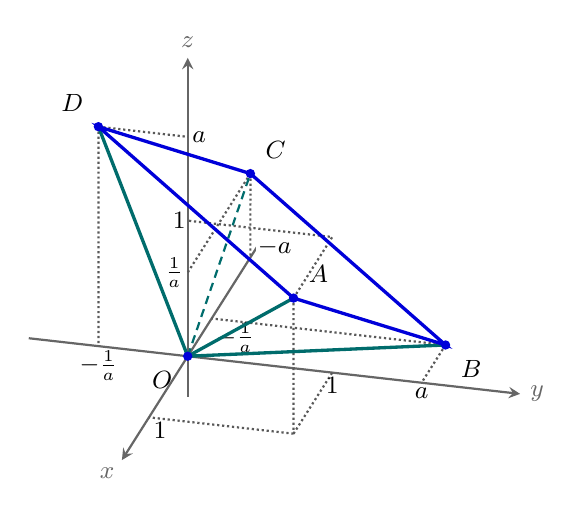
\begin{tikzpicture}[x={(-0.2588cm,-0.4082cm)}, y={(0.9659cm,-0.1094cm)}, z={(0.0000cm,0.9063cm)}, scale=1.9, >=stealth,
      every node/.style={font=\small}]
      \pgfmathsetmacro{\gold}{(1+sqrt(5))/2}
      \pgfmathsetmacro{\ig}{1/\gold}
      \coordinate (O) at (0,0,0);
      \coordinate (A) at (1,1,1);
      \coordinate (B) at (-\ig,\gold,0);
      \coordinate (C) at (-\gold,0,\ig);
      \coordinate (D) at (0,-\ig,\gold);
      \coordinate (A0) at (1,1,0); % A の xy 平面への正射影
      % 座標軸
      \draw[->, thick, gray!80!black] (-1.9,0,0) -- (1.7,0,0) node[below left=-1pt] {$x$};
      \draw[->, thick, gray!80!black] (0,-1.1,0) -- (0,2.3,0) node[right] {$y$};
      \draw[->, thick, gray!80!black] (0,0,-0.3) -- (0,0,2.2) node[above] {$z$};
      % 各頂点から座標軸への点線
      \begin{scope}[densely dotted, thick, gray!70!black]
        \draw (A) -- (A0) (A0) -- (1,0,0) (A0) -- (0,1,0) (A) -- (0,1,1) -- (0,0,1);
        \draw (B) -- (-\ig,0,0) (B) -- (0,\gold,0);
        \draw (C) -- (-\gold,0,0) (C) -- (0,0,\ig);
        \draw (D) -- (0,-\ig,0) (D) -- (0,0,\gold);
      \end{scope}
      % 軸上の座標
      \begin{scope}[font=\footnotesize, inner sep=1.5pt]
        \node[below right] at (1,0,0) {$1$};
        \node[below right] at (-\ig,0,0) {$-\frac{1}{a}$};
        \node[above right, xshift=2pt, fill=white, inner sep=0.5pt] at (-\gold,0,0) {$-a$};
        \node[below] at (0,1,0) {$1$};
        \node[below] at (0,\gold,0) {$a$};
        \node[below] at (0,-\ig,0) {$-\frac{1}{a}$};
        \node[left] at (0,0,\ig) {$\frac{1}{a}$};
        \node[left, fill=white, inner sep=0.5pt] at (0,0,1) {$1$};
        \node[right] at (0,0,\gold) {$a$};
      \end{scope}
      % 四角錐 O-ABCD（O-C は隠れ線）
      \draw[densely dashed, thick, teal!85!black] (O) -- (C);
      \draw[very thick, teal!85!black] (O) -- (A) (O) -- (B) (O) -- (D);
      \draw[very thick, blue!85!black] (A) -- (B) -- (C) -- (D) -- cycle;
      \foreach \p/\pos in {O/below left, A/above right, B/below right, C/above right, D/above left}{
        \node[circle, fill=blue!85!black, inner sep=1.2pt] at (\p) {};
        \node[\pos=2pt] at (\p) {$\p$};
      }
    \end{tikzpicture}
    \caption{四角錐$O$-$ABCD$と各頂点の座標}
    \label{1992-6:fig:pyramid}
  \end{figure}

  A$(1,1,1)$, B$(-\dfrac{1}{a},a,0)$, C$(-a,0,\dfrac{1}{a})$, D$(0,\dfrac{-1}{a},a)$である．

  \paragraph{(1)}
  題意を示すには，$|AB|=|AD|=|DC|$であることと，$\angle BAD = \angle ADC = \dfrac{\pi}{2}$であることを示せば良い．
  各辺をなすベクトルは
  \begin{align}
    \overrightarrow{\text{AB}} & = \mqty( -\dfrac{1}{a}-1 \\ a-1 \\ -1) \\
    \overrightarrow{\text{AD}} & = \mqty( -1             \\ -\dfrac{1}{a}-1 \\ a-1 ) \\
    \overrightarrow{\text{DC}} & = \mqty(-a              \\ \dfrac{1}{a} \\ \dfrac{1}{a}-a )
  \end{align}
  となる．

  まず辺の長さについて，
  \begin{align}
    |\overrightarrow{\text{AB}}|
    & = |\overrightarrow{\text{AD}}|                                                   \\
    & = \sqrt{1+(a-1)^2+\left(-\dfrac{1}{a}-1\right)^2}                      \\
    & = \sqrt{a^2 -2a + 3 + \dfrac{2}{a} + \dfrac{1}{a^2}}                    \\
    & = \sqrt{\left(a-\dfrac{1}{a}\right)^2 - 2\left(a-\dfrac{1}{a}\right)+5}
  \end{align}
  であり，
  \begin{align}
    a-\dfrac{1}{a}
    & = \dfrac{1+\sqrt{5}}{2} - \dfrac{2}{1+\sqrt{5}}
    = 1 \label{eq:1}
  \end{align}
  を代入すると
  \begin{align}
    |\overrightarrow{\text{AB}}| = |\overrightarrow{\text{AD}}|   = 2
  \end{align}
  である．ついで
  \begin{align}
    |\overrightarrow{\text{DC}}|
    & = \sqrt{a^2+\dfrac{1}{a^2}+\left(\dfrac{1}{a}-a\right)^2} \\
    & = \sqrt{2\left(a-\dfrac{1}{a}\right)^2+2}                \\
    & = 2
  \end{align}
  だから，
  \begin{align}
    |\overrightarrow{\text{AB}}| = |\overrightarrow{\text{AD}}| =|\overrightarrow{\text{DC}}| = 2
  \end{align}
  となる．

  次に角度については，ベクトルの内積が$0$になれば良い．
  \cref{eq:1}を利用すると，
  \begin{align}
    \overrightarrow{\text{AB}} \cdot \overrightarrow{\text{AD}}
    & = 1+\dfrac{1}{a} + (a-1)\left(-\dfrac{1}{a}-1\right) -(a-1)                    \\
    & = 2\left(\dfrac{1}{a}-a+1\right)                                              \\
    & = 0                                                                          \\
    \overrightarrow{\text{AD}} \cdot \overrightarrow{\text{DC}} & = a + \dfrac{1}{a}\left(-\dfrac{1}{a}-1\right)+(a-1)\left(\dfrac{1}{a}-a\right) \\
    & = 2a - \dfrac{1}{a^2} - \dfrac{2}{a} +1 -a^2                                   \\
    & = 2\left(a-\dfrac{1}{a}\right) - \left(a-\dfrac{1}{a}\right)^2 -1              \\
    & = 0
  \end{align}
  より，確かに内積は$0$であり，
  \begin{align}
    \angle BAD = \angle ADC = \dfrac{\pi}{2}
  \end{align}
  である．

  以上から，$\text{ABCD}$は一辺の長さ$2$の正方形である．$\cdots$(答)

  \paragraph{(2)}
  点OとDは平面$x=0$上にあり，点AとBは平面$x=0$を挟んで両側に存在する．
  そこで，辺ABと平面$x=0$の交点を求める．
  辺ABの方程式は
  \begin{align}
    \mqty(x \\ y \\ z) = \mqty(1 \\ 1 \\ 1) + t \mqty(-\dfrac{1}{a}-1 \\ a-1 \\ -1)
  \end{align}
  だから，$x=0$を代入して，交点を表す$t$は
  \begin{align}
    t
    & = \dfrac{1}{1/a+1} \\
    & = \dfrac{a}{a+1}
  \end{align}
  である．従ってこの交点をEとすると，EはABを
  \begin{align}
    t: 1-t & = \dfrac{a}{a+1}: \dfrac{1}{a+1}
  \end{align}
  に内分する点であり，(1)より$|AB|=2$だから
  \begin{align}
    |AE| & = \dfrac{2a}{a+1} \\
    |EB| & = \dfrac{2}{a+1}
  \end{align}
  である．この様子を\cref{1992-6:fig:1}に示す．

  \begin{figure}[H]
    \centering
    \begin{tikzpicture}[scale=2.0]
      % 正方形 ABCD の頂点
      \coordinate (A) at (0,0);
      \coordinate (B) at (2,0);
      \coordinate (C) at (2,2);
      \coordinate (D) at (0,2);
      \coordinate (E) at (1.2,0);

      % 正方形の辺を描画
      \draw (A) -- (B) -- (C) -- (D) -- cycle;

      % 線分 DE を描画
      \draw (D) -- (E);

      % 頂点のラベル
      \node [below left] at (A) {A};
      \node [below right] at (B) {B};
      \node [above right] at (C) {C};
      \node [above left] at (D) {D};
      \node [below] at (E) {E};

      % 比率のラベル
      \node [below=0.3cm] at (0.6,0) {$\frac{2a}{a+1}$};
      \node [below=0.3cm] at (1.6,0) {$\frac{2}{a+1}$};
    \end{tikzpicture}
    \caption{四角形ABCDの様子}
    \label{1992-6:fig:1}
  \end{figure}

  題意の$W_1, W_2$ は各々 $\triangle \text{ADE}$, $\square \text{EBCD}$を底面とし，
  高さは同じ立体だから体積比は底面積比に等しく，
  求める体積の比は
  \begin{align}
    W_1:W_2
    & = (\triangle \text{ADE}) : (\square \text{EBCD}) \\
    & = \text{|AE|} : (\text{|EB|}+\text{|CD|})        \\
    & = \dfrac{2a}{a+1} : \left(\dfrac{2}{a+1}+2\right) \\
    & = a : a+2                                      \\
    & = 1:\sqrt{5}
  \end{align}
  である．$\cdots$(答)

  {\bf [解説]}
  \begin{figure}[H]
    \centering
    \tdplotsetmaincoords{70}{120}
    \begin{tikzpicture}[tdplot_main_coords, scale=1.5,
      every node/.style={font=\small}]
      \pgfmathsetmacro{\gold}{(1+sqrt(5))/2}
      \coordinate (O) at (0,0,0);
      \coordinate (A) at (1,1,1);
      \coordinate (B) at ({-1/\gold},\gold,0);
      \coordinate (C) at (-\gold,0,{1/\gold});
      \coordinate (D) at (0,{-1/\gold},\gold);
      \coordinate (E) at ($(A)!{\gold/(\gold+1)}!(B)$);
      \fill[pattern=north east lines,pattern color=red!55]
      (A) -- (E) -- (D) -- cycle;
      \fill[pattern=north west lines,pattern color=blue!55]
      (E) -- (B) -- (C) -- (D) -- cycle;
      \draw[very thick,blue!85!black] (A) -- (B) -- (C) -- (D) -- cycle;
      \draw[very thick,teal!85!black] (O) -- (A) (O) -- (B) (O) -- (D);
      \draw[densely dashed,thick,gray!70!black] (O) -- (C);
      \draw[thick,red!85!black] (D) -- (E);
      \foreach \p/\pos in {O/below left,A/below left,B/below right,C/above right,D/above left,E/above right}{
        \node[circle,fill=blue!85!black,inner sep=1.2pt] at (\p) {};
        \node[fill=white,inner sep=1pt,\pos=3pt] at (\p) {$\p$};
      }
    \end{tikzpicture}
    \caption{平面$x=0$で切った四角錐$O$-$ABCD$（切り口は三角形$ODE$）}
    \label{1992-6:fig:2}
  \end{figure}

  \newpage
\end{multicols}
\end{document}
